\scanpage{25}

% All text is in one manuscript hand. The anchored layout keeps the two long
% rules beside/through the writing, and keeps the p247 interlinear material
% at its observed level. Coordinates follow the supplied whole image.
\figure{%
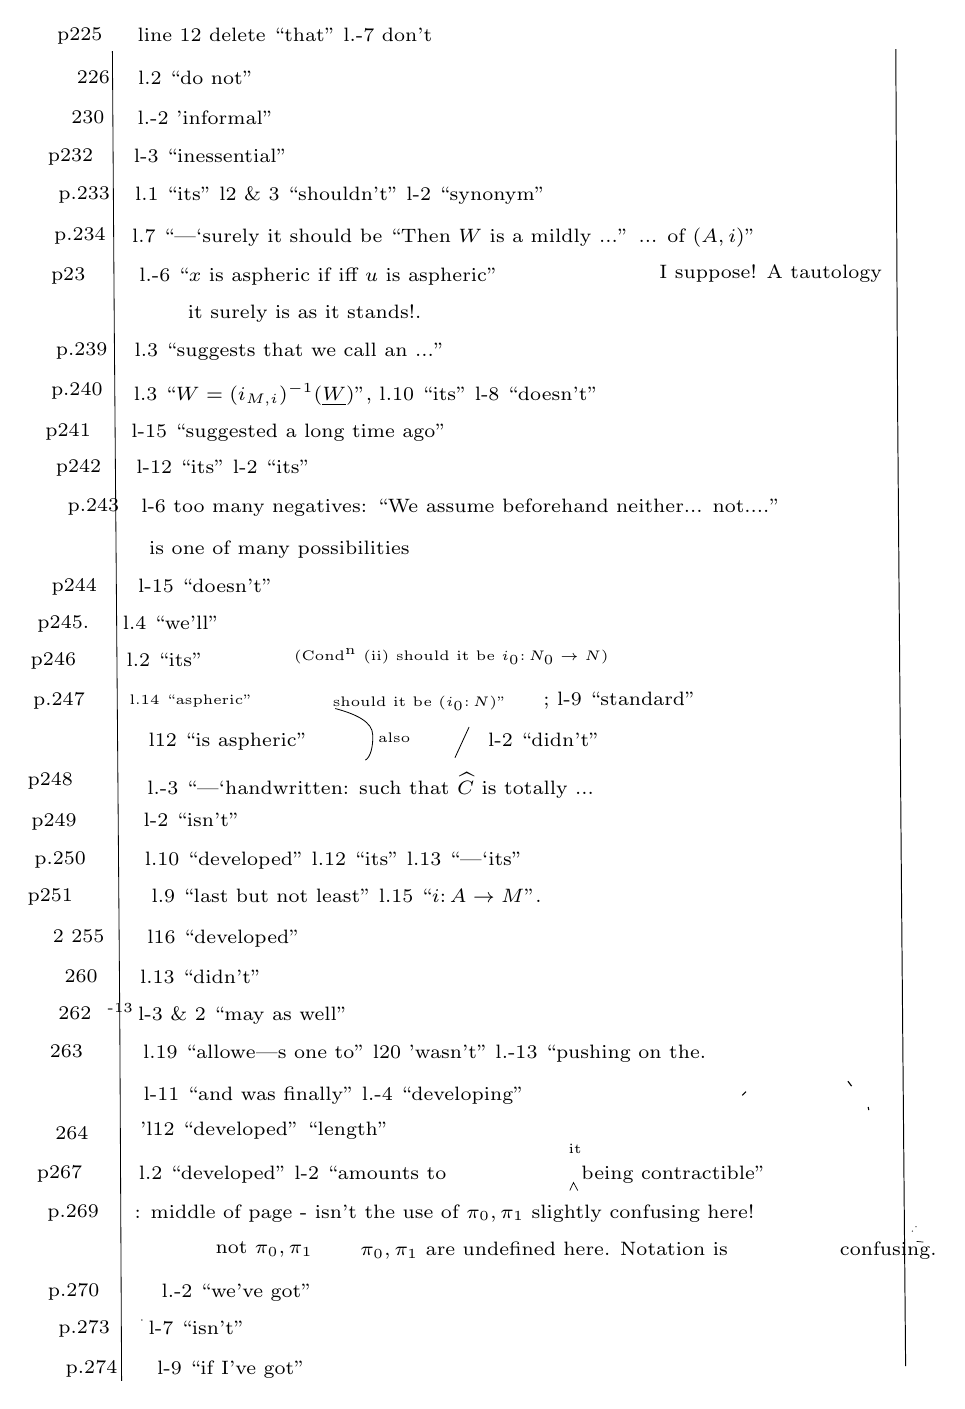
\begin{tikzpicture}[x=0.0078cm,y=-0.0078cm,
  every node/.style={anchor=north west,inner sep=0pt,outer sep=0pt,font=\scriptsize}]
% BEGIN left_rule
\draw[line width=0.30pt] (232,97) -- (235,538) -- (240,1165) -- (244,1668) -- (247,2263);
% END left_rule
% BEGIN right_rule
\draw[line width=0.35pt] (1508,94) -- (1511,682) -- (1517,1433) -- (1524,2239);
% END right_rule

% BEGIN p225
\node at (142,59) {p225};
\node at (273,59) {line 12 delete ``that'' l.-7 don't};
% END p225

% BEGIN p226
\node at (174,130) {226};
\node at (274,130) {l.2 ``do not''};
% END p226

% BEGIN p230
\node at (165,195) {230};
\node at (273,195) {l.-2 'informal''};
% END p230

% BEGIN p232
\node at (127,256) {p232};
\node at (267,256) {l-3 ``inessential''};
% END p232

% BEGIN p233
\node at (144,319) {p.233};
\node at (269,319) {l.1 ``its'' l2 \& 3 ``shouldn't'' l-2 ``synonym''};
% END p233

% BEGIN p234a
\node at (137,385) {p.234};
\node at (264,385) {l.7 \unsure{``|`}surely it should be ``Then $W$ is a mildly ...\deleted{\unsure{''}} ... of $(A,i)$''};
% END p234a

% BEGIN p234b
\node at (132,451) {\deleted{p23}};
\node at (276,451) {l.-6 ``$x$ is aspheric \deleted{\unsure{if}} iff $u$ is aspheric''};
\node at (1123,445) {I suppose! A tautology};
\node at (355,511) {it surely is as it stands!.};
% END p234b

% BEGIN p239
\node at (140,573) {p.239};
\node at (268,573) {l.3 ``suggests that we call an ...''};
% END p239

% BEGIN p240
\node at (132,638) {p.240};
\node at (267,638) {l.3 ``$W=(i_{M,i})^{-1}(\underline{W})$'', l.10 ``its'' l-8 ``doesn't''};
% END p240

% BEGIN p241
\node at (123,705) {p241};
\node at (263,705) {l-15 ``suggested a long time ago''};
% END p241

% BEGIN p242
\node at (140,764) {p242};
\node at (271,764) {l-12 ``its'' l-2 ``its''};
% END p242

% BEGIN p243
\node at (159,826) {p.243};
\node at (279,826) {l-6 too many negatives: ``We assume beforehand neither... not....''};
\node at (292,896) {is one of many possibilities};
% END p243

% BEGIN p244
\node at (133,957) {p244};
\node at (274,957) {l-15 ``doesn't''};
% END p244

% BEGIN p245
\node at (110,1017) {p245.};
\node at (249,1017) {l.4 ``we'll''};
% END p245

% BEGIN p246
\node at (99,1078) {p246};
\node at (255,1078) {l.2 ``its''};
% END p246

% BEGIN p247
\node at (103,1142) {p.247};
\node[font=\tiny] at (260,1145) {\deleted{l.14 ``\unsure{aspheric}''}};
\node[font=\tiny] at (528,1071) {\inserted{(Cond\textsuperscript{n} (ii) should it be $i_0\colon N_0\to N$)}};
\node[font=\tiny] at (591,1148) {\deleted{should it be $(i_{\unsure{0}}\colon N)$\unsure{''}}};
\node at (934,1141) {; l-9 ``standard''};
\node at (291,1208) {l12 ``is aspheric''};
\node[font=\tiny] at (665,1208) {\inserted{also}};
\node at (844,1208) {l-2 ``didn't''};
% BEGIN p247_connectors
\draw[line width=0.30pt] (595,1168) .. controls (629,1177) and (656,1190) .. (656,1211)
  .. controls (657,1230) and (652,1248) .. (644,1252);
\draw[line width=0.30pt] (813,1198) -- (790,1248);
% END p247_connectors
% END p247

% BEGIN p248
\node at (94,1273) {p248};
\node at (289,1273) {l.-3 \unsure{``|`}\uline{handwritten}: such that $\widehat C$ \uline{is} totally ...};
% END p248

% BEGIN p249
\node at (100,1339) {p249};
\node at (283,1339) {l-2 ``isn't''};
% END p249

% BEGIN p250
\node at (105,1401) {p.250};
\node at (285,1401) {l.10 ``developed'' l.12 ``its'' l.13 \unsure{``|`}its''};
% END p250

% BEGIN p251
\node at (94,1462) {p251};
\node at (296,1462) {l.9 ``last but not least'' l.15 ``$i\colon A\to M$''.};
% END p251

% BEGIN p255
\node at (135,1529) {\deleted{2} 255};
\node at (289,1529) {l16 ``developed''};
% END p255

% BEGIN p260
\node at (154,1594) {260};
\node at (277,1594) {l.13 ``didn't''};
% END p260

% BEGIN p262
\node at (144,1654) {262};
\node[font=\tiny] at (224,1649) {-\deleted{\unsure{13}}};
\node at (274,1654) {l-3 \& 2 ``may as well''};
% END p262

% BEGIN p263
\node at (130,1716) {263};
\node at (282,1716) {l.19 ``allow\unsure{e|s} one to'' l20 'wasn't'' l.-13 ``pushing on the.};
\node at (283,1784) {l-11 ``and was finally'' l.-4 ``developing''};
% BEGIN p263_marks
\draw[line width=0.40pt] (1258,1798) -- (1264,1792);
\draw[line width=0.40pt] (1430,1775) -- (1436,1783);
\draw[line width=0.40pt] (1463,1817) -- (1464,1822);
% END p263_marks
% END p263

% BEGIN p264
\node at (139,1849) {264};
\node at (277,1842) {'l12 ``developed'' ``length''};
% END p264

% BEGIN p267
\node at (109,1913) {p267};
\node at (275,1913) {l.2 ``developed'' l-2 ``amounts to};
\node[font=\tiny] at (975,1878) {\inserted{it}};
\node at (996,1913) {being contractible''};
\draw[line width=0.25pt] (977,1953) -- (983,1940) -- (990,1953);
% END p267

% BEGIN p269
\node at (126,1976) {p.269};
\node at (268,1976) {: middle of page - \deleted{isn't the use of $\pi_0,\pi_1$ slightly confusing here!}};
\node at (400,2037) {\deleted{not $\pi_0,\pi_1$}};
\node at (636,2037) {$\pi_0,\pi_1$ are undefined \uline{here}. Notation is};
\node at (1417,2037) {confusing.};
% BEGIN p269_marks
\fill (1535,2019) circle[radius=0.08mm];
\fill (1541,2012) circle[radius=0.08mm];
\draw[line width=0.25pt] (1542,2036) -- (1553,2037);
% END p269_marks
% END p269

% BEGIN p270
\node at (127,2106) {p.270};
\node at (312,2106) {l.-2 ``we've got''};
% END p270

% BEGIN p273
\node at (144,2166) {p.273};
\node at (291,2166) {l-7 ``isn't''};
% BEGIN p273_point
\fill (280,2164) circle[radius=0.09mm];
% END p273_point
% END p273

% BEGIN p274
\node at (156,2231) {p.274};
\node at (305,2231) {l-9 ``if I've got''};
% END p274
\end{tikzpicture}%
}

% archive sheet number: 24
% Two circular pale marks near the right paper edge are physical sheet features,
% not mathematical drawings or text. No manuscript page number is present.
